% !TEX root = ../main.tex

\chapter*{附录B\hskip.5em 其他附录文本}
\addcontentsline{toc}{chapter}{附录B\hskip.5em 其他附录文本}
% 设置章节编号为1,即A
\setcounter{chapter}{2}
% 重置所有计数器
\setcounter{equation}{0}
\setcounter{figure}{0}
\setcounter{table}{0}

\lipsum[2]

\section*{B.1\hskip.5em 求和算子}

\textbf{求和算子} 是用以表达多个数求和运算的一个缩略符号,它在统计学和计量经济学分析中扮演着重要作用。如果 $\{x_i: i=1, 2, \cdots, n\}$ 表示 $n$ 个数的一个序列,那么我们就把这 $n$ 个数的和写为\equref{eq:2}:
\begin{equation}
\label{eq:2}
a^2+b^2=c^2
\end{equation}

引用图片示例:\figref{appen:fire}

\begin{figure}[!htbp]
	\centering
	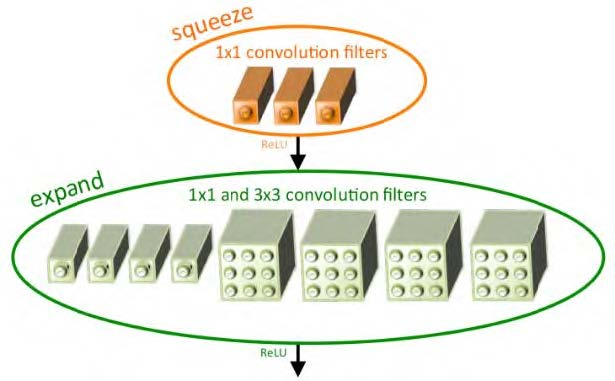
\includegraphics[width=0.6\textwidth]{less3}
	\caption{附录插图示例:f\/ire模块}
     \label{appen:fire}
\end{figure}